\documentclass[11pt]{article}
%Zur Einbingung von Grafiken
\usepackage{graphicx}

%Deutsche Bezeichnungen des Inhaltsverzeichnis, Abbildungsverzeichnis usw.
\usepackage[german]{babel}

%Um Grafiken anzeigen zu lassen, wo sie im tex File geschrieben wurden. \begin{figure}[H]
\usepackage{float}

%Syntax Highlighting
\usepackage{minted}

\usepackage[autostyle,german=quotes]{csquotes}

%Fuer Hintergrundbilder
\usepackage{eso-pic}

%Bilder Transparent machen
\usepackage{transparent}

%Fallunterscheidungen wie etwa gerade und ungerade Seiten
\usepackage{ifthen}

\addbibresource{lit/lit.bib}
\parindent 0ex
\begin{document}

%\AddToShipoutPicture{
%  \ifthenelse{
%    \isodd{
%        \value{page}
%    }
%  }
%  {%zum Gap entfernen das Kommentar
%    \transparent{0.2}\includegraphics[width=\paperwidth, height=\paperheight]{img/bild1.jpg}
%  }
%  {%zum Gap entfernen das Kommentar
%    \transparent{1}\includegraphics[width=\paperwidth, height=\paperheight]{img/bild1.jpg}
%  }  
%}

\begin{center}
    
\includegraphics[width=0.5\paperwidth]{img/hs-harz.png}

    \vspace{20mm}

    \Huge
    \textsc{Hausarbeit}

    \vspace{5mm}

    \Large
    \textsc{Es handelt sich um Untertitel}
    \normalsize
    \vfill
    Vorgelegt von

    \textbf{Niclas Schmidt}
    Meine Adresse:

    \vspace{20mm}

    \begin{tabular}{r c}
        Erstprüfer: & Prof. Jürgen Singer Ph. D.\\
        Zweitprüfer: & Daniel Ackermann \\
        Datum: & 02.11.2020
    \end{tabular}
    
    \vspace{5mm}
\end{center}

\tableofcontents
\newpage
\listoffigures
\newpage
%listoflistings umbennen in Listingverzeichnis
\renewcommand*{\listoflistingscaption}{Listingverzeichnis}
\listoflistings
\newpage
\section{Erstes Kapitel}
hier kommt Text hin.
Lorem ipsum dolor sit amet, consectetuer adipiscing elit. Aenean commodo ligula eget dolor. Aenean massa. Cum sociis natoque penatibus et magnis dis parturient montes, nascetur ridiculus mus. Donec quam felis, ultricies nec, pellentesque eu, pretium quis, sem. Nulla consequat massa quis enim. Donec pede justo, fringilla vel, aliquet nec, vulputate eget, arcu. In enim justo, rhoncus ut, imperdiet a, venenatis vitae, justo. Nullam dictum felis eu pede mollis pretium. Integer tincidunt. Cras dapibus. Vivamus elementum semper nisi. Aenean vulputate eleifend tellus. Aenean leo ligula, porttitor eu, consequat vitae, eleifend ac, enim. Aliquam lorem ante, dapibus in, viverra quis, feugiat a, tellus. Phasellus viverra nulla ut metus varius laoreet. Quisque rutrum. Aenean imperdiet. Etiam ultricies nisi vel augue. Curabitur ullamcorper ultricies nisi. Nam eget dui. Etiam rhoncus. Maecenas tempus, tellus eget condimentum rhoncus, sem quam semper libero, sit amet adipiscing sem neque sed ipsum. Nam quam nunc, blandit vel, luctus pulvinar, hendrerit id, lorem. Maecenas nec odio et ante tincidunt tempus. Donec vitae sapien ut libero venenatis faucibus. Nullam quis ante. Etiam sit amet orci eget eros faucibus tincidunt.

Aenean commodo ligula eget dolor. Aenean massa. Cum sociis natoque penatibus et magnis dis parturient montes, nascetur ridiculus mus. Donec quam felis, ultricies nec, pellentesque eu, pretium quis, sem. Nulla consequat massa quis enim. Donec pede justo, fringilla vel, aliquet nec, vulputate eget, arcu. In enim justo, rhoncus ut, imperdiet a, venenatis vitae, justo. Nullam dictum felis eu pede mollis pretium. Integer tincidunt. Cras dapibus. Vivamus elementum semper nisi. 
\begin{listing}[H]
    \caption{Beispiel Javacode}
    \label{lst:mein_quelltext}
    \begin{minted}[
        linenos,
        numbersep=5pt,
        frame=lines,
        framesep=5pt
    ]{java}
    public static void main(String[] args){
        String s = "Hallo"
        System.out.println(s);
    }
    \end{minted}
\end{listing}

\subsection{Erstes Unterkapitel}
hier kommt Unterkapiteltext hin und referenziert \ref{lst:mein_quelltext} \nameref{lst:mein_quelltext}
Hier wird aus einem Buch verwiesen: verwiesener Text \footnote{Vgl. \cite[S. 190]{teller1994visibility}} .
\begin{quote}
    ich zitiere Text aus einem Buch. \footnote{Vgl. \cite[S. 190]{wiki:Fußball}}
\end{quote}
Ich möchte noch auf ein Bild aus dem Anhang verweisen. siehe Anhang \ref{lab:erster_anhang} Abbildung \ref{fig:anhang_blume}.
\subsubsection{Erstes Unter-Unter-Kapitel}
hier kommt Unter-Unter-Kapiteltext hin.

\paragraph{Erster Paragraph}
hier kommt Paragraphtext.

\subparagraph{Erster Unter-Paragraph}
hier kommt fetter \textbf{Unter-Paragraphtext}.
hier kommt krusiver \textit{Unter-Paragraphtext}.

%Windowstaste Punkt
hier kommt zitierter „Unter-Paragraphtext“. 
hier kommt zitierter \enquote{Unter-Paragraphtext}

\section{Zweites Kapitel}

Diese Abbildung \ref{fig: Blume} \nameref{fig: Blume} zeigt eine Blume.

\begin{figure}[H]
    \centering
    \includegraphics[width=0.75\textwidth]{img/bild1.jpg}
    \caption[Blume]{Blume in Gras mit Seifenblasen}
    \label{fig: Blume}
\end{figure}
hier kommt weiterer Text hin.
alles geklappt!
Diese Abbildung \ref{fig: Blume} zeigt eine Blume.

siehe \nameref{lab:eidessstattliche_erklaerung}.

\printbibliography
%\include{content/eidesstattliche_erklaerung/eidesstattliche_erklärung}

%Hintergrundbild fuer Eidessstattliche Erklärung entfernen
%\ClearShipoutPicture
%setcounter -> Zahl vor Inhaltsverzeichnis weg bei Eidesstattliche Erklärung
\setcounter{secnumdepth}{0}
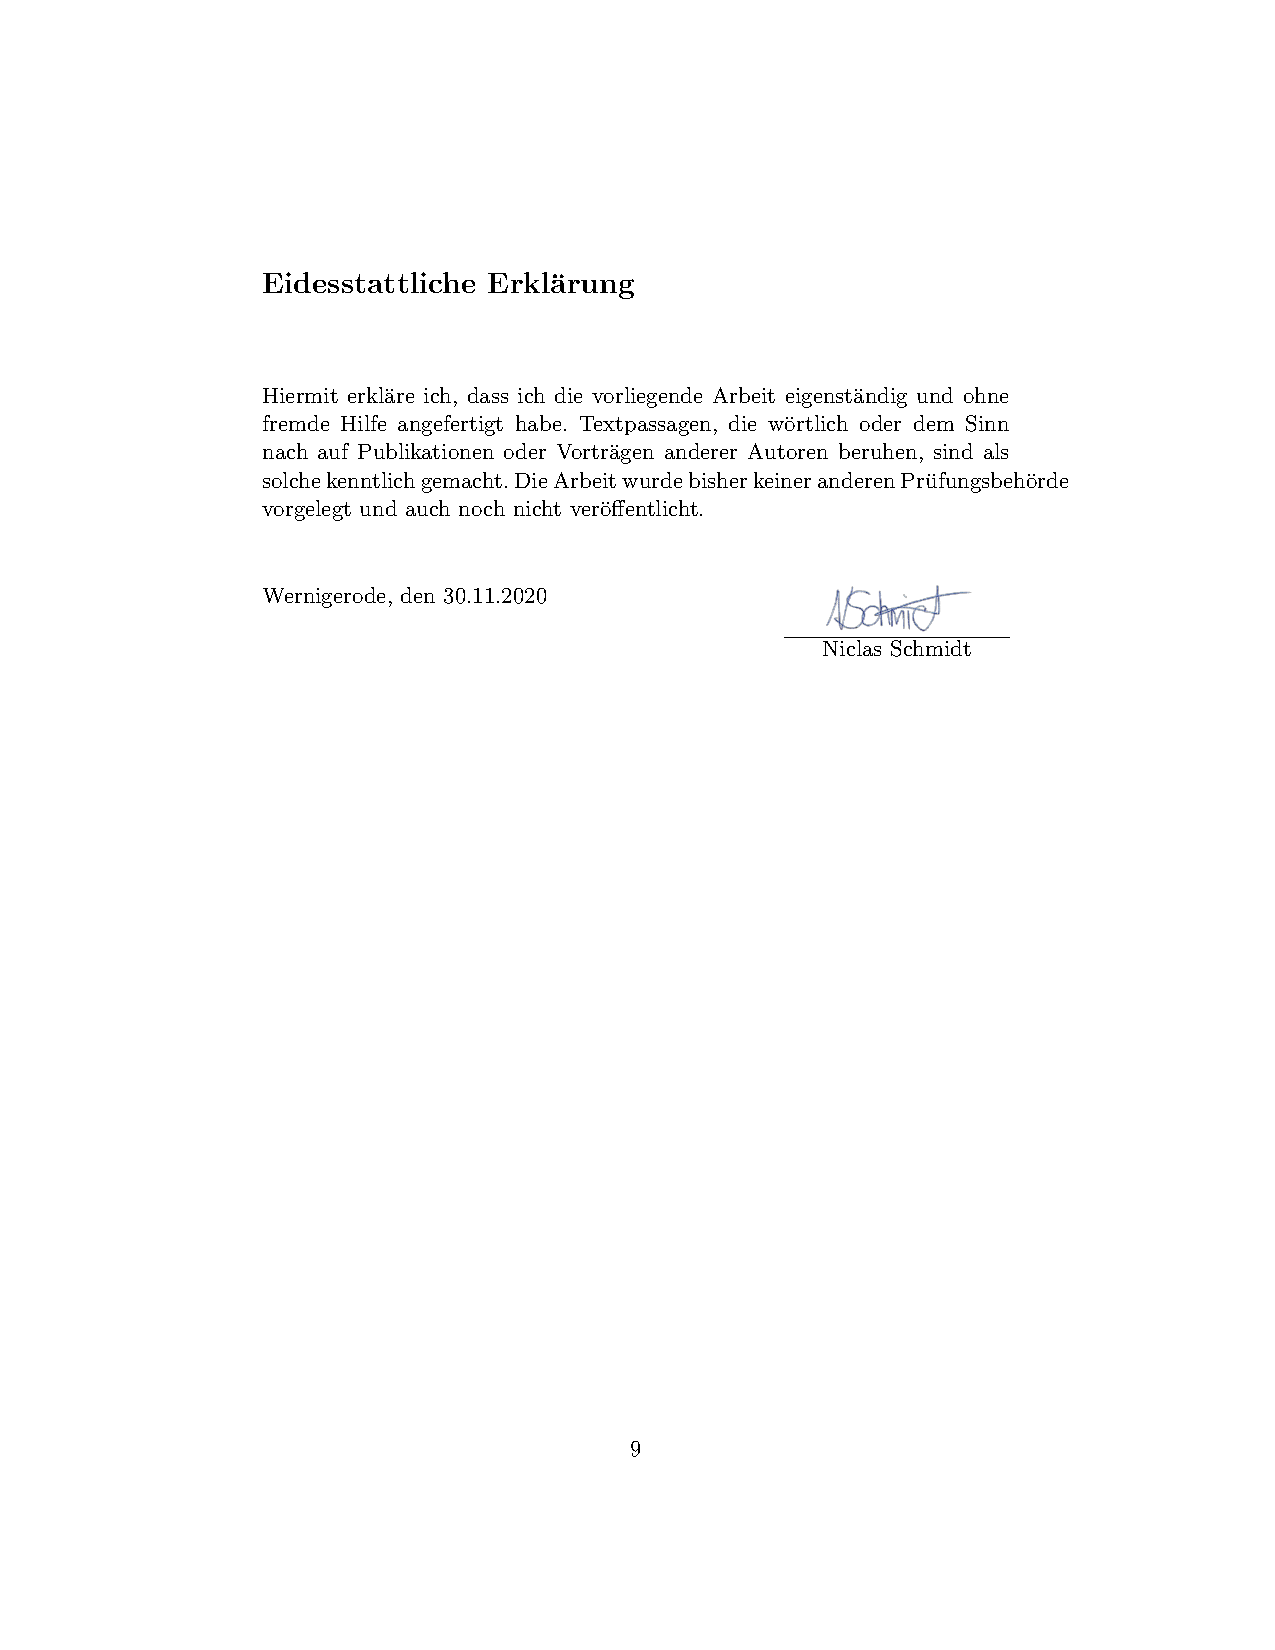
\includepdf[
    addtotoc={
        1, % page number
        section, % section oder subsection...
        1, % level, 1 fuer sections...
        Eidesstattliche Erklärung, % heading, Titel in TOC
        lab:eidessstattliche_erklaerung% \ref
    }
]{signiert.pdf}


\end{document}
